%  LaTeX support: latex@mdpi.com
%  In case you need support, please attach all files that are necessary for compiling as well as the log file, and specify the details of your LaTeX setup (which operating system and LaTeX version / tools you are using).

%=================================================================
\documentclass[mathematics,article,submit,moreauthors,pdftex]{mdpi}

% If you would like to post an early version of this manuscript as a preprint, you may use preprint as the journal and change 'submit' to 'accept'. The document class line would be, e.g., \documentclass[preprints,article,accept,moreauthors,pdftex]{mdpi}. This is especially recommended for submission to arXiv, where line numbers should be removed before posting. For preprints.org, the editorial staff will make this change immediately prior to posting.

%% Some pieces required from the pandoc template
\setlist[itemize]{leftmargin=*,labelsep=5.8mm}
\setlist[enumerate]{leftmargin=*,labelsep=4.9mm}


%--------------------
% Class Options:
%--------------------
%----------
% journal
%----------
% Choose between the following MDPI journals:
% acoustics, actuators, addictions, admsci, aerospace, agriculture, agriengineering, agronomy, algorithms, animals, antibiotics, antibodies, antioxidants, applsci, arts, asc, asi, atmosphere, atoms, axioms, batteries, bdcc, behavsci , beverages, bioengineering, biology, biomedicines, biomimetics, biomolecules, biosensors, brainsci , buildings, cancers, carbon , catalysts, cells, ceramics, challenges, chemengineering, chemistry, chemosensors, children, cleantechnol, climate, clockssleep, cmd, coatings, colloids, computation, computers, condensedmatter, cosmetics, cryptography, crystals, dairy, data, dentistry, designs , diagnostics, diseases, diversity, drones, econometrics, economies, education, electrochem, electronics, energies, entropy, environments, epigenomes, est, fermentation, fibers, fire, fishes, fluids, foods, forecasting, forests, fractalfract, futureinternet, futurephys, galaxies, games, gastrointestdisord, gels, genealogy, genes, geohazards, geosciences, geriatrics, hazardousmatters, healthcare, heritage, highthroughput, horticulturae, humanities, hydrology, ijerph, ijfs, ijgi, ijms, ijns, ijtpp, informatics, information, infrastructures, inorganics, insects, instruments, inventions, iot, j, jcdd, jcm, jcp, jcs, jdb, jfb, jfmk, jimaging, jintelligence, jlpea, jmmp, jmse, jnt, jof, joitmc, jpm, jrfm, jsan, land, languages, laws, life, literature, logistics, lubricants, machines, magnetochemistry, make, marinedrugs, materials, mathematics, mca, medicina, medicines, medsci, membranes, metabolites, metals, microarrays, micromachines, microorganisms, minerals, modelling, molbank, molecules, mps, mti, nanomaterials, ncrna, neuroglia, nitrogen, notspecified, nutrients, ohbm, particles, pathogens, pharmaceuticals, pharmaceutics, pharmacy, philosophies, photonics, physics, plants, plasma, polymers, polysaccharides, preprints , proceedings, processes, proteomes, psych, publications, quantumrep, quaternary, qubs, reactions, recycling, religions, remotesensing, reports, resources, risks, robotics, safety, sci, scipharm, sensors, separations, sexes, signals, sinusitis, smartcities, sna, societies, socsci, soilsystems, sports, standards, stats, surfaces, surgeries, sustainability, symmetry, systems, technologies, test, toxics, toxins, tropicalmed, universe, urbansci, vaccines, vehicles, vetsci, vibration, viruses, vision, water, wem, wevj

%---------
% article
%---------
% The default type of manuscript is "article", but can be replaced by:
% abstract, addendum, article, benchmark, book, bookreview, briefreport, casereport, changes, comment, commentary, communication, conceptpaper, conferenceproceedings, correction, conferencereport, expressionofconcern, extendedabstract, meetingreport, creative, datadescriptor, discussion, editorial, essay, erratum, hypothesis, interestingimages, letter, meetingreport, newbookreceived, obituary, opinion, projectreport, reply, retraction, review, perspective, protocol, shortnote, supfile, technicalnote, viewpoint
% supfile = supplementary materials

%----------
% submit
%----------
% The class option "submit" will be changed to "accept" by the Editorial Office when the paper is accepted. This will only make changes to the frontpage (e.g., the logo of the journal will get visible), the headings, and the copyright information. Also, line numbering will be removed. Journal info and pagination for accepted papers will also be assigned by the Editorial Office.

%------------------
% moreauthors
%------------------
% If there is only one author the class option oneauthor should be used. Otherwise use the class option moreauthors.

%---------
% pdftex
%---------
% The option pdftex is for use with pdfLaTeX. If eps figures are used, remove the option pdftex and use LaTeX and dvi2pdf.

%=================================================================
\firstpage{1}
\makeatletter
\setcounter{page}{\@firstpage}
\makeatother
\pubvolume{xx}
\issuenum{1}
\articlenumber{5}
\pubyear{2019}
\copyrightyear{2019}
%\externaleditor{Academic Editor: name}
\history{Received: date; Accepted: date; Published: date}
\updates{yes} % If there is an update available, un-comment this line

%% MDPI internal command: uncomment if new journal that already uses continuous page numbers
%\continuouspages{yes}

%------------------------------------------------------------------
% The following line should be uncommented if the LaTeX file is uploaded to arXiv.org
%\pdfoutput=1

%=================================================================
% Add packages and commands here. The following packages are loaded in our class file: fontenc, calc, indentfirst, fancyhdr, graphicx, lastpage, ifthen, lineno, float, amsmath, setspace, enumitem, mathpazo, booktabs, titlesec, etoolbox, amsthm, hyphenat, natbib, hyperref, footmisc, geometry, caption, url, mdframed, tabto, soul, multirow, microtype, tikz

%=================================================================
%% Please use the following mathematics environments: Theorem, Lemma, Corollary, Proposition, Characterization, Property, Problem, Example, ExamplesandDefinitions, Hypothesis, Remark, Definition
%% For proofs, please use the proof environment (the amsthm package is loaded by the MDPI class).

%=================================================================
% Full title of the paper (Capitalized)
\Title{Check your outliers! An introduction to identifying statistical
outliers in R with \emph{easystats}}

% Authors, for the paper (add full first names)
\Author{Rémi
Thériault$^{1,*}$\href{https://orcid.org/0000-0003-4315-6788}{\orcidicon}, Mattan
S.
Ben-Shachar$^{2}$\href{https://orcid.org/0000-0002-4287-4801}{\orcidicon}, Indrajeet
Patil$^{3}$\href{https://orcid.org/0000-0003-1995-6531}{\orcidicon}, Daniel
Lüdecke$^{4}$\href{https://orcid.org/0000-0002-8895-3206}{\orcidicon}, Brenton
M.
Wiernik$^{5}$\href{https://orcid.org/0000-0001-9560-6336}{\orcidicon}, Dominique
Makowski$^{6}$\href{https://orcid.org/0000-0001-5375-9967}{\orcidicon}}

% Authors, for metadata in PDF
\AuthorNames{Rémi Thériault, Mattan S. Ben-Shachar, Indrajeet
Patil, Daniel Lüdecke, Brenton M. Wiernik, Dominique Makowski}

% Affiliations / Addresses (Add [1] after \address if there is only one affiliation.)
\address{%
$^{1}$ \quad Department of Psychology, Université du Québec à Montréal,
Montréal, Québec, Canada; \\
$^{2}$ \quad Independent Researcher; \\
$^{3}$ \quad Center for Humans and Machines, Max Planck Institute for
Human Development, Berlin, Germany; \\
$^{4}$ \quad Institute of Medical Sociology, University Medical Center
Hamburg-Eppendorf, Germany; \\
$^{5}$ \quad Independent Researcher, Tampa, FL, USA; \\
$^{6}$ \quad School of Psychology, University of Sussex, Brighton,
UK; \\
}
% Contact information of the corresponding author
\corres{Correspondence: \href{mailto:theriault.remi@courrier.uqam.ca}{\nolinkurl{theriault.remi@courrier.uqam.ca}}.}

% Current address and/or shared authorship








% The commands \thirdnote{} till \eighthnote{} are available for further notes

% Simple summary
\simplesumm{The \emph{\{performance\}} package from the \emph{easystats}
ecosystem makes it easy to diagnose outliers in R and according to
current best practices thanks to the \texttt{check\_outiers()}
function.}

% Abstract (Do not insert blank lines, i.e. \\)
\abstract{Beyond the challenge of keeping up-to-date with current best
practices regarding the diagnosis and treatment of outliers, an
additional difficulty arises concerning the mathematical implementation
of the recommended methods. In this paper, we provide an overview of
current recommandations and best practices and demonstrate how they can
easily and conveniently be implemented in the R statistical computing
software, using the \emph{\{performance\}} package of the
\emph{easystats} ecosystem. We cover univariate, multivariate, and
model-based statistical outlier detection methods, their recommended
threshold, standard output, and plotting methods. We conclude with
recommendations on the handling of outliers: the different theoretical
types of outliers, whether to exclude or winsorize them, and the
importance of transparency.}

% Keywords
\keyword{univariate outliers; multivariate outliers; robust detection
methods; R; easystats}

% The fields PACS, MSC, and JEL may be left empty or commented out if not applicable
%\PACS{J0101}
%\MSC{}
%\JEL{}

%%%%%%%%%%%%%%%%%%%%%%%%%%%%%%%%%%%%%%%%%%
% Only for the journal Diversity
%\LSID{\url{http://}}

%%%%%%%%%%%%%%%%%%%%%%%%%%%%%%%%%%%%%%%%%%
% Only for the journal Applied Sciences:
%\featuredapplication{Authors are encouraged to provide a concise description of the specific application or a potential application of the work. This section is not mandatory.}
%%%%%%%%%%%%%%%%%%%%%%%%%%%%%%%%%%%%%%%%%%

%%%%%%%%%%%%%%%%%%%%%%%%%%%%%%%%%%%%%%%%%%
% Only for the journal Data:
%\dataset{DOI number or link to the deposited data set in cases where the data set is published or set to be published separately. If the data set is submitted and will be published as a supplement to this paper in the journal Data, this field will be filled by the editors of the journal. In this case, please make sure to submit the data set as a supplement when entering your manuscript into our manuscript editorial system.}

%\datasetlicense{license under which the data set is made available (CC0, CC-BY, CC-BY-SA, CC-BY-NC, etc.)}

%%%%%%%%%%%%%%%%%%%%%%%%%%%%%%%%%%%%%%%%%%
% Only for the journal Toxins
%\keycontribution{The breakthroughs or highlights of the manuscript. Authors can write one or two sentences to describe the most important part of the paper.}

%\setcounter{secnumdepth}{4}
%%%%%%%%%%%%%%%%%%%%%%%%%%%%%%%%%%%%%%%%%%

% Pandoc syntax highlighting
\usepackage{color}
\usepackage{fancyvrb}
\newcommand{\VerbBar}{|}
\newcommand{\VERB}{\Verb[commandchars=\\\{\}]}
\DefineVerbatimEnvironment{Highlighting}{Verbatim}{commandchars=\\\{\}}
% Add ',fontsize=\small' for more characters per line
\usepackage{framed}
\definecolor{shadecolor}{RGB}{248,248,248}
\newenvironment{Shaded}{\begin{snugshade}}{\end{snugshade}}
\newcommand{\AlertTok}[1]{\textcolor[rgb]{0.94,0.16,0.16}{#1}}
\newcommand{\AnnotationTok}[1]{\textcolor[rgb]{0.56,0.35,0.01}{\textbf{\textit{#1}}}}
\newcommand{\AttributeTok}[1]{\textcolor[rgb]{0.77,0.63,0.00}{#1}}
\newcommand{\BaseNTok}[1]{\textcolor[rgb]{0.00,0.00,0.81}{#1}}
\newcommand{\BuiltInTok}[1]{#1}
\newcommand{\CharTok}[1]{\textcolor[rgb]{0.31,0.60,0.02}{#1}}
\newcommand{\CommentTok}[1]{\textcolor[rgb]{0.56,0.35,0.01}{\textit{#1}}}
\newcommand{\CommentVarTok}[1]{\textcolor[rgb]{0.56,0.35,0.01}{\textbf{\textit{#1}}}}
\newcommand{\ConstantTok}[1]{\textcolor[rgb]{0.00,0.00,0.00}{#1}}
\newcommand{\ControlFlowTok}[1]{\textcolor[rgb]{0.13,0.29,0.53}{\textbf{#1}}}
\newcommand{\DataTypeTok}[1]{\textcolor[rgb]{0.13,0.29,0.53}{#1}}
\newcommand{\DecValTok}[1]{\textcolor[rgb]{0.00,0.00,0.81}{#1}}
\newcommand{\DocumentationTok}[1]{\textcolor[rgb]{0.56,0.35,0.01}{\textbf{\textit{#1}}}}
\newcommand{\ErrorTok}[1]{\textcolor[rgb]{0.64,0.00,0.00}{\textbf{#1}}}
\newcommand{\ExtensionTok}[1]{#1}
\newcommand{\FloatTok}[1]{\textcolor[rgb]{0.00,0.00,0.81}{#1}}
\newcommand{\FunctionTok}[1]{\textcolor[rgb]{0.00,0.00,0.00}{#1}}
\newcommand{\ImportTok}[1]{#1}
\newcommand{\InformationTok}[1]{\textcolor[rgb]{0.56,0.35,0.01}{\textbf{\textit{#1}}}}
\newcommand{\KeywordTok}[1]{\textcolor[rgb]{0.13,0.29,0.53}{\textbf{#1}}}
\newcommand{\NormalTok}[1]{#1}
\newcommand{\OperatorTok}[1]{\textcolor[rgb]{0.81,0.36,0.00}{\textbf{#1}}}
\newcommand{\OtherTok}[1]{\textcolor[rgb]{0.56,0.35,0.01}{#1}}
\newcommand{\PreprocessorTok}[1]{\textcolor[rgb]{0.56,0.35,0.01}{\textit{#1}}}
\newcommand{\RegionMarkerTok}[1]{#1}
\newcommand{\SpecialCharTok}[1]{\textcolor[rgb]{0.00,0.00,0.00}{#1}}
\newcommand{\SpecialStringTok}[1]{\textcolor[rgb]{0.31,0.60,0.02}{#1}}
\newcommand{\StringTok}[1]{\textcolor[rgb]{0.31,0.60,0.02}{#1}}
\newcommand{\VariableTok}[1]{\textcolor[rgb]{0.00,0.00,0.00}{#1}}
\newcommand{\VerbatimStringTok}[1]{\textcolor[rgb]{0.31,0.60,0.02}{#1}}
\newcommand{\WarningTok}[1]{\textcolor[rgb]{0.56,0.35,0.01}{\textbf{\textit{#1}}}}

% tightlist command for lists without linebreak
\providecommand{\tightlist}{%
  \setlength{\itemsep}{0pt}\setlength{\parskip}{0pt}}

% From pandoc table feature
\usepackage{longtable,booktabs,array}
\usepackage{calc} % for calculating minipage widths
% Correct order of tables after \paragraph or \subparagraph
\usepackage{etoolbox}
\makeatletter
\patchcmd\longtable{\par}{\if@noskipsec\mbox{}\fi\par}{}{}
\makeatother
% Allow footnotes in longtable head/foot
\IfFileExists{footnotehyper.sty}{\usepackage{footnotehyper}}{\usepackage{footnote}}
\makesavenoteenv{longtable}



\begin{document}


%%%%%%%%%%%%%%%%%%%%%%%%%%%%%%%%%%%%%%%%%%

\hypertarget{introduction}{%
\section{Introduction}\label{introduction}}

Real-life data often contain observations that can be considered
\emph{abnormal} when compared to the main population. The cause of
it---be it because they belong to a different distribution (originating
from a different generative process) or simply being extreme cases,
statistically rare but not impossible---can be hard to assess, and the
boundaries of ``abnormal'' are hard to define.

Nonetheless, the improper handling of these outliers can substantially
affect statistical model estimations, biasing effect estimations and
weakening the models' predictive performance. It is thus essential to
address this problem in a thoughtful manner. Yet, despite the existence
of established recommendations and guidelines, many researchers still do
not treat outliers in a consistent manner, or do so using inappropriate
strategies \citep{simmons2011false, leys2013outliers}.

One possible reason is that researchers are not aware of the existing
recommendations, or do not know how to implement them using their
analysis software. In this paper, we show how to follow current best
practices for automatic and reproducible statistical outlier detection
(SOD) using R and the \emph{\{performance\}} package
\citep{ludecke2021performance}, which is part of the \emph{easystats}
ecosystem of packages that build an R framework for easy statistical
modeling, visualization, and reporting \citep{easystatspackage}.

\hypertarget{identifying-outliers}{%
\section{Identifying Outliers}\label{identifying-outliers}}

Although many researchers attempt to identify outliers with measures
based on the mean (e.g., \emph{z} scores), those methods are problematic
because the mean and standard deviation themselves are not robust to the
influence of outliers and they assume normally distribute data (i.e., a
Gaussian distribution). Therefore, current guidelines recommend using
robust methods to identify outliers, such as those relying on the median
as opposed to the mean
\citep{leys2019outliers, leys2013outliers, leys2018outliers}.

Nonetheless, which exact outlier method to use depends on many factors.
In some cases, eye-gauging odd observations can be an appropriate
solution, though many researchers will favour algorithmic solutions to
detect potential outliers, for example, based on a continuous value
expressing the observation stands out from the others.

One of the factors to consider when selecting an algorithmic outlier
detection method is the statistical test of interest. When using a
regression model, relevant information can be found by identifying
observations that do not fit well with the model. This approach, known
as model-based outliers detection (as outliers are extracted after the
statistical model has been fit), can be contrasted with
distribution-based outliers detection, which is based on the distance
between an observation and the ``center'' of its population. Various
quantification strategies of this distance exist for the latter, both
univariate (involving only one variable at a time) or multivariate
(involving multiple variables).

When no method is readily available to detect model-based outliers, such
as for structural equation modelling (SEM), looking for multivariate
outliers may be of relevance. For simple tests (\emph{t} tests or
correlations) that compare values of the same variable, it can be
appropriate to check for univariate outliers. However, univariate
methods can give false positives since \emph{t} tests and correlations,
ultimately, are also models/multivariable statistics. They are in this
sense more limited, but we show them nonetheless for educational
purposes.

Importantly, whatever approach researchers choose remains a subjective
decision, which usage (and rationale) must be transparently documented
and reproducible \citep{leys2019outliers}. Researchers should commit
(ideally in a preregistration) to an outlier treatment method before
collecting the data. They should report in the paper their decisions and
details of their methods, as well as any deviation from their original
plan. These transparency practices can help reduce false positives due
to excessive researchers' degrees of freedom (i.e., choice flexibility
throughout the analysis). In the following section, we will go through
each of the mentioned methods and provide examples on how to implement
them with R.

\hypertarget{univariate-outliers}{%
\subsection{Univariate Outliers}\label{univariate-outliers}}

Researchers frequently attempt to identify outliers using measures of
deviation from the center of a variable's distribution. One of the most
popular such procedure is the \emph{z} score transformation, which
computes the distance in standard deviation (SD) from the mean. However,
as mentioned earlier, this popular method is not robust. Therefore, for
univariate outliers, it is recommended to use the median along with the
Median Absolute Deviation (MAD), which are more robust than the
interquartile range or the mean and its standard deviation
\citep{leys2019outliers, leys2013outliers}.

Researchers can identify outliers based on robust (i.e., MAD-based)
\emph{z} scores using the \texttt{check\_outliers()} function of the
\emph{\{performance\}} package, by specifying
\texttt{method\ =\ "zscore\_robust"}.\footnote{Note that
  \texttt{check\_outliers()} only checks numeric variables.} Although
\citet{leys2013outliers} suggest a default threshold of 2.5 and
\citet{leys2019outliers} a threshold of 3, \emph{\{performance\}} uses
by default a less conservative threshold of
\textasciitilde3.29.\footnote{3.29 is an approximation of the two-tailed
  critical value for \emph{p} \textless{} .001, obtained through
  \texttt{qnorm(p\ =\ 1\ -\ 0.001\ /\ 2)}. We chose this threshold for
  consistency with the thresholds of all our other methods.} That is,
data points will be flagged as outliers if they go beyond +/-
\textasciitilde3.29 MAD. Users can adjust this threshold using the
\texttt{threshold} argument, as demonstrated below.

\begin{Shaded}
\begin{Highlighting}[]
\FunctionTok{library}\NormalTok{(performance)}

\CommentTok{\# Create some artificial outliers and an ID column}
\NormalTok{data }\OtherTok{\textless{}{-}} \FunctionTok{rbind}\NormalTok{(mtcars[}\DecValTok{1}\SpecialCharTok{:}\DecValTok{4}\NormalTok{], }\DecValTok{42}\NormalTok{, }\DecValTok{55}\NormalTok{)}
\NormalTok{data }\OtherTok{\textless{}{-}} \FunctionTok{cbind}\NormalTok{(}\AttributeTok{car =} \FunctionTok{row.names}\NormalTok{(data), data)}

\NormalTok{outliers }\OtherTok{\textless{}{-}} \FunctionTok{check\_outliers}\NormalTok{(data, }\AttributeTok{method =} \StringTok{"zscore\_robust"}\NormalTok{, }\AttributeTok{ID =} \StringTok{"car"}\NormalTok{)}
\NormalTok{outliers}
\end{Highlighting}
\end{Shaded}

\begin{verbatim}
#> 2 outliers detected: cases 33, 34.
#> - Based on the following method and threshold: zscore_robust (3.09).
#> - For variables: mpg, cyl, disp, hp.
#> 
#> -----------------------------------------------------------------------------
#>  
#> The following observations were considered outliers for two or more
#>   variables by at least one of the selected methods:
#> 
#>   Row car n_Zscore_robust
#> 1  33  33               2
#> 2  34  34               2
#> 
#> -----------------------------------------------------------------------------
#> Outliers per variable (zscore_robust): 
#> 
#> $mpg
#>    Row car Distance_Zscore_robust
#> 33  33  33               3.709699
#> 34  34  34               5.848328
#> 
#> $cyl
#>    Row car Distance_Zscore_robust
#> 33  33  33               12.14083
#> 34  34  34               16.52502
\end{verbatim}

The row numbers of the detected outliers can be obtained by using
\texttt{which()} on the output object, which can be used for exclusions
for example:

\begin{Shaded}
\begin{Highlighting}[]
\FunctionTok{which}\NormalTok{(outliers)}
\end{Highlighting}
\end{Shaded}

\begin{verbatim}
#> [1] 33 34
\end{verbatim}

\begin{Shaded}
\begin{Highlighting}[]
\NormalTok{data\_clean }\OtherTok{\textless{}{-}}\NormalTok{ data[}\SpecialCharTok{{-}}\FunctionTok{which}\NormalTok{(outliers), ]}
\end{Highlighting}
\end{Shaded}

All \texttt{check\_outliers()} output objects possess a \texttt{plot()}
method, meaning it is also possible to visualize the outliers:

\begin{Shaded}
\begin{Highlighting}[]
\FunctionTok{library}\NormalTok{(see)}

\FunctionTok{plot}\NormalTok{(outliers)}
\end{Highlighting}
\end{Shaded}

\begin{figure}
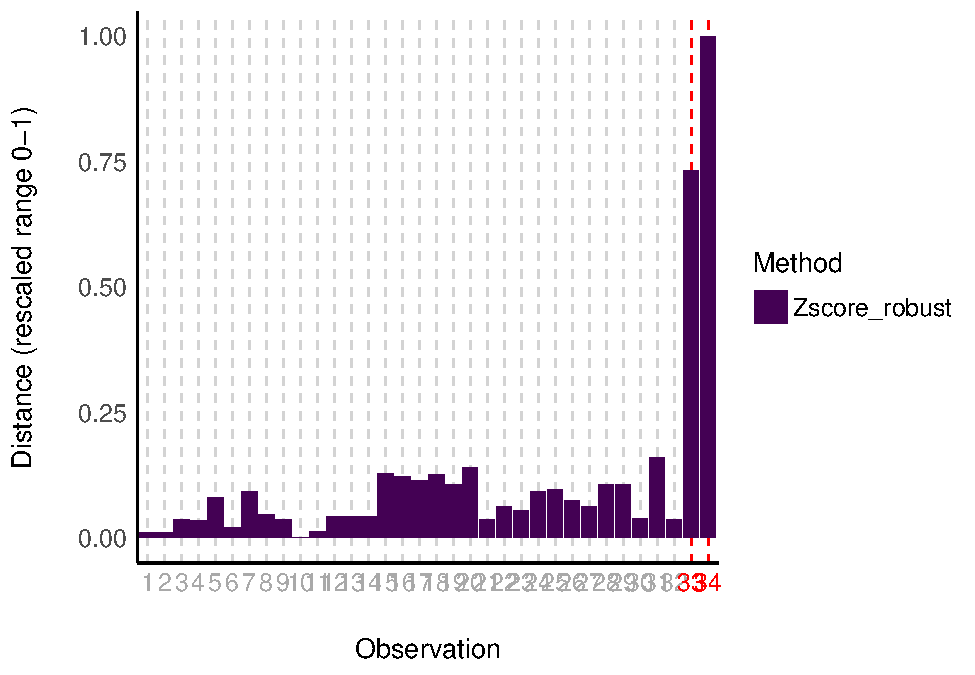
\includegraphics[width=1\linewidth]{paper_files/figure-latex/univariate-1} \caption{Visual depiction of outliers using the robust z-score method.}\label{fig:univariate}
\end{figure}

Other univariate methods are available, such as using the interquartile
range (IQR), or based on different intervals, such as the Highest
Density Interval (HDI) or the Bias Corrected and Accelerated Interval
(BCI). These methods are documented and described in the function's
\href{https://easystats.github.io/performance/reference/check_outliers.html}{help
page}.

\hypertarget{multivariate-outliers}{%
\subsection{Multivariate Outliers}\label{multivariate-outliers}}

Univariate outliers can be useful when the focus is on a particular
variable, for instance the reaction time, as extreme values might be
indicative of inattention or non-task-related behavior\footnote{ Note
  that they might not be the optimal way of treating reaction time
  outliers \citep{ratcliff1993methods, van1995statistical}}.

However, in many scenarios, variables of a data set are not independent,
and an abnormal observation will impact multiple dimensions. For
instance, a participant giving random answers to a questionnaire. In
this case, computing the \emph{z} score for each of the questions might
not lead to satisfactory results. Instead, one might want to look at
these variables together.

One common approach for this is to compute multivariate distance metrics
such as the Mahalanobis distance. Although the Mahalanobis distance is
very popular, just like the regular \emph{z} scores method, it is not
robust and is heavily influenced by the outliers themselves. Therefore,
for multivariate outliers, it is recommended to use the Minimum
Covariance Determinant, a robust version of the Mahalanobis distance
\citep[MCD,][]{leys2018outliers, leys2019outliers}.

In \emph{\{performance\}}'s \texttt{check\_outliers()}, one can use this
approach with \texttt{method\ =\ "mcd"}.\footnote{Our default threshold
  for the MCD method is defined by
  \texttt{stats::qchisq(p\ =\ 1\ -\ 0.001,\ df\ =\ ncol(x))}, which
  again is an approximation of the critical value for \emph{p}
  \textless{} .001 consistent with the thresholds of our other methods.}

\begin{Shaded}
\begin{Highlighting}[]
\NormalTok{outliers }\OtherTok{\textless{}{-}} \FunctionTok{check\_outliers}\NormalTok{(data, }\AttributeTok{method =} \StringTok{"mcd"}\NormalTok{)}
\NormalTok{outliers}
\end{Highlighting}
\end{Shaded}

\begin{verbatim}
#> 9 outliers detected: cases 7, 15, 16, 17, 24, 29, 31, 33, 34.
#> - Based on the following method and threshold: mcd (20).
#> - For variables: mpg, cyl, disp, hp.
\end{verbatim}

\begin{Shaded}
\begin{Highlighting}[]
\FunctionTok{plot}\NormalTok{(outliers)}
\end{Highlighting}
\end{Shaded}

\begin{figure}
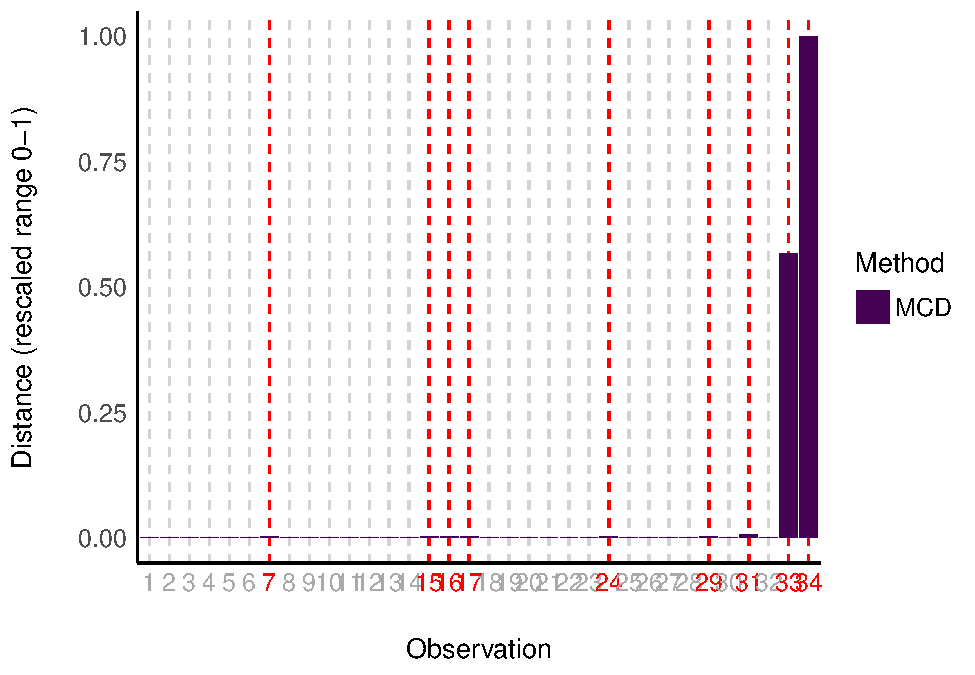
\includegraphics[width=1\linewidth]{paper_files/figure-latex/multivariate-1} \caption{Visual depiction of outliers using the Minimum Covariance Determinant (MCD) method, a robust version of the Mahalanobis distance.}\label{fig:multivariate}
\end{figure}

Other multivariate methods are available, such as another type of robust
Mahalanobis distance that in this case relies on an orthogonalized
Gnanadesikan-Kettenring pairwise estimator
\citep{gnanadesikan1972robust}. These methods are documented and
described in the function's
\href{https://easystats.github.io/performance/reference/check_outliers.html}{help
page}.

\hypertarget{model-based-outliers}{%
\subsection{Model-Based Outliers}\label{model-based-outliers}}

Working with regression models creates the possibility of using
model-based SOD methods. These methods rely on the concept of
\emph{leverage}, that is, how much influence a given observation can
have on the model estimates. If few observations have a relatively
strong leverage/influence on the model, one can suspect that the model's
estimates are biased by these observations, in which case flagging them
as outliers could prove helpful (see next section, ``Handling
Outliers'').

In \{performance\}, two such model-based SOD methods are currently
available: Cook's distance, for regular regression models, and Pareto,
for Bayesian models. As such, \texttt{check\_outliers()} can be applied
directly on regression model objects, by simply specifying
\texttt{method\ =\ "cook"} (or \texttt{method\ =\ "pareto"} for Bayesian
models).\footnote{Our default threshold for the Cook method is defined
  by \texttt{stats::qf(0.5,\ ncol(x),\ nrow(x)\ -\ ncol(x))}, which
  again is an approximation of the critical value for \emph{p}
  \textless{} .001 consistent with the thresholds of our other methods.}

\begin{Shaded}
\begin{Highlighting}[]
\NormalTok{model }\OtherTok{\textless{}{-}} \FunctionTok{lm}\NormalTok{(disp }\SpecialCharTok{\textasciitilde{}}\NormalTok{ mpg }\SpecialCharTok{*}\NormalTok{ disp, }\AttributeTok{data =}\NormalTok{ data)}
\NormalTok{outliers }\OtherTok{\textless{}{-}} \FunctionTok{check\_outliers}\NormalTok{(model, }\AttributeTok{method =} \StringTok{"cook"}\NormalTok{)}
\NormalTok{outliers}
\end{Highlighting}
\end{Shaded}

\begin{verbatim}
#> 1 outlier detected: case 34.
#> - Based on the following method and threshold: cook (0.708).
#> - For variable: (Whole model).
\end{verbatim}

\begin{Shaded}
\begin{Highlighting}[]
\FunctionTok{plot}\NormalTok{(outliers)}
\end{Highlighting}
\end{Shaded}

\begin{figure}
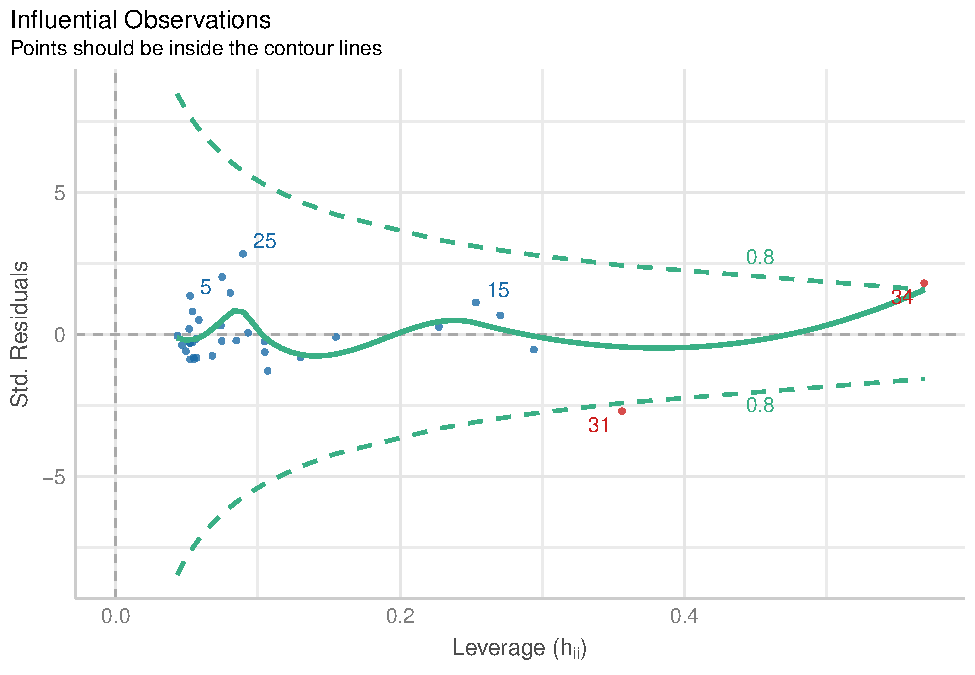
\includegraphics[width=1\linewidth]{paper_files/figure-latex/model-1} \caption{Visual depiction of outliers based on Cook's distance (leverage and standardized residuals).}\label{fig:model}
\end{figure}

Table 1 below summarizes which methods to use in which cases, and with
what threshold.

\begin{longtable}[]{@{}
  >{\raggedright\arraybackslash}p{(\columnwidth - 4\tabcolsep) * \real{0.3506}}
  >{\raggedright\arraybackslash}p{(\columnwidth - 4\tabcolsep) * \real{0.3161}}
  >{\raggedright\arraybackslash}p{(\columnwidth - 4\tabcolsep) * \real{0.3333}}@{}}
\caption{Summary of Statistical Outlier Detection Methods
Recommendations.}\tabularnewline
\toprule()
\begin{minipage}[b]{\linewidth}\raggedright
Statistical Test
\end{minipage} & \begin{minipage}[b]{\linewidth}\raggedright
Diagnosis Method
\end{minipage} & \begin{minipage}[b]{\linewidth}\raggedright
Recommended Threshold
\end{minipage} \\
\midrule()
\endfirsthead
\toprule()
\begin{minipage}[b]{\linewidth}\raggedright
Statistical Test
\end{minipage} & \begin{minipage}[b]{\linewidth}\raggedright
Diagnosis Method
\end{minipage} & \begin{minipage}[b]{\linewidth}\raggedright
Recommended Threshold
\end{minipage} \\
\midrule()
\endhead
Supported regression model & \textbf{Model-based}: Cook (or Pareto for
Bayesian models) & \texttt{qf(0.5,\ ncol(x),\ nrow(x)\ -\ ncol(x))} (or
0.7 for Pareto) \\
Structural Equation Modeling (or other unsupported model) &
\textbf{Multivariate}: Minimum Covariance Determinant (MCD) &
\texttt{qchisq(p\ =\ 1\ -\ 0.001,\ df\ =\ ncol(x))} \\
Simple test with few variables (\emph{t} test, correlation, etc.) &
\textbf{Univariate}: robust \emph{z} scores (MAD) &
\texttt{qnorm(p\ =\ 1\ -\ 0.001\ /\ 2)}, \textasciitilde{} 3.29 \\
\bottomrule()
\end{longtable}

\hypertarget{cooks-distance-vs.-mcd}{%
\subsubsection{Cook's Distance vs.~MCD}\label{cooks-distance-vs.-mcd}}

\citet{leys2018outliers} report a preference for the MCD method over
Cook's distance. This is because Cook's distance removes one observation
at a time and checks its corresponding influence on the model each time
\citep{cook1977detection}, and flags any observation that has a large
influence. In the view of these authors, when there are several
outliers, the process of removing a single outlier at a time is
problematic as the model remains ``contaminated'' or influenced by other
possible outliers in the model, rendering this method suboptimal in the
presence of multiple outliers.

However, distribution-based approaches are not a silver bullet either,
and there are cases where the usage of methods agnostic to theoretical
and statistical models of interest might be problematic. For example, a
very tall person would be expected to also be much heavier than average,
but that would still fit with the expected association between height
and weight (i.e., it would be in line with a model such as
\texttt{weight\ \textasciitilde{}\ height}). In contrast, using
multivariate outlier detection methods there may flag this person as
being an outlier---being unusual on two variables, height and
weight---even though the pattern fits perfectly with our predictions.

Furthermore, unusual observations happen naturally: extreme observations
are expected even when taken from a normal distribution. While
statistical models can integrate this ``expectation'', multivariate
outlier methods might be too conservative, flagging too many
observations despite belonging to the right generative process. For
these reasons, we believe that model-based methods are still preferable
to the MCD when using supported regression models. Additionally, if the
presence of multiple outliers is a significant concern, regression
methods that are more robust to outliers should be considered---like
\emph{t} regression or quantile regression---as they render their
precise identification less critical.

\hypertarget{multiple-methods}{%
\subsection{Multiple Methods}\label{multiple-methods}}

An alternative approach that is possible is to combine several methods,
based on the assumption that different methods provide different angles
of looking at the problem. By applying a variety of methods, one can
hope to ``triangulate'' the true outliers (those consistently flagged by
multiple methods) and thus attempt to minimize false positives.

In practice, this approach computes a composite outlier score, formed of
the average of the binary (0 or 1) classification results of each
method. It represents the probability that each observation is
classified as an outlier by at least one method. The default decision
rule classifies rows with composite outlier scores superior or equal to
0.5 as outlier observations (i.e., that were classified as outliers by
at least half of the methods). In \emph{\{performance\}}'s
\texttt{check\_outliers()}, one can use this approach by including all
desired methods in the corresponding argument.

\begin{Shaded}
\begin{Highlighting}[]
\NormalTok{outliers }\OtherTok{\textless{}{-}} \FunctionTok{check\_outliers}\NormalTok{(model, }\AttributeTok{method =} \FunctionTok{c}\NormalTok{(}\StringTok{"zscore\_robust"}\NormalTok{, }\StringTok{"mcd"}\NormalTok{, }\StringTok{"cook"}\NormalTok{))}
\NormalTok{outliers}
\end{Highlighting}
\end{Shaded}

\begin{verbatim}
#> 2 outliers detected: cases 33, 34.
#> - Based on the following methods and thresholds: zscore_robust (3.09),
#>   mcd (0.708), cook (13.816).
#> - For variable: (Whole model).
#> 
#> Note: Outliers were classified as such by at least half of the selected methods. 
#> 
#> -----------------------------------------------------------------------------
#>  
#> The following observations were considered outliers for two or more
#>   variables by at least one of the selected methods:
#> 
#>   Row n_Zscore_robust          n_MCD         n_Cook
#> 1  33               1 (Multivariate)              0
#> 2  34               1 (Multivariate) (Multivariate)
#> 3  20               0 (Multivariate)              0
\end{verbatim}

\begin{Shaded}
\begin{Highlighting}[]
\FunctionTok{plot}\NormalTok{(outliers)}
\end{Highlighting}
\end{Shaded}

\begin{figure}
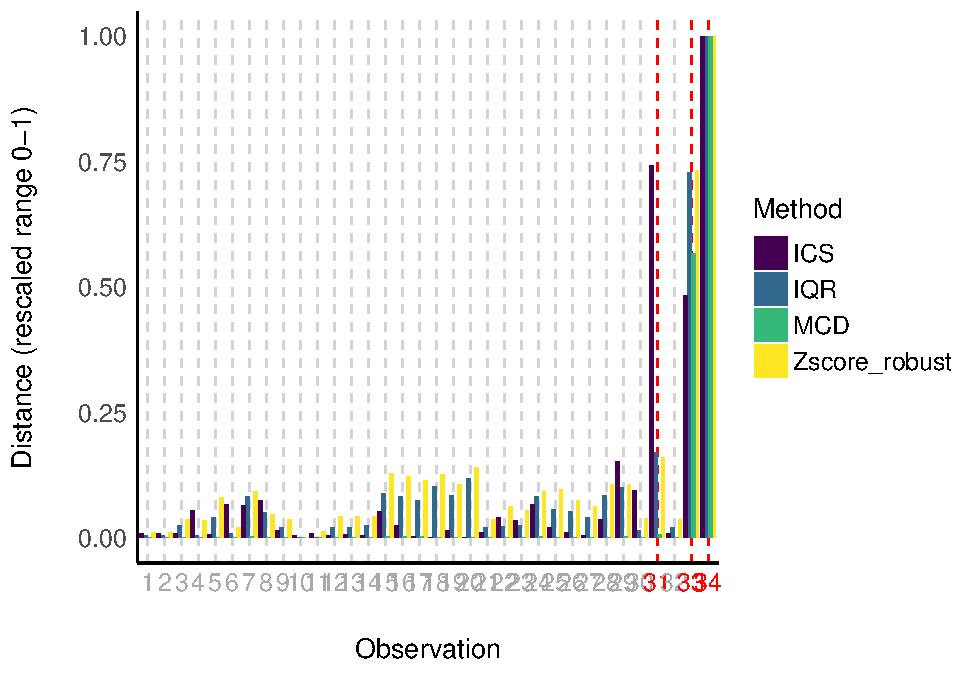
\includegraphics[width=1\linewidth]{paper_files/figure-latex/multimethod-1} \caption{Visual depiction of outliers using several different statistical outlier detection methods.}\label{fig:multimethod}
\end{figure}

Outliers (counts or per variables) for individual methods can then be
obtained through attributes. For example:

\begin{Shaded}
\begin{Highlighting}[]
\FunctionTok{attributes}\NormalTok{(outliers)}\SpecialCharTok{$}\NormalTok{outlier\_var}\SpecialCharTok{$}\NormalTok{zscore\_robust}
\end{Highlighting}
\end{Shaded}

\begin{verbatim}
#> $mpg
#>    Row Distance_Zscore_robust
#> 33  33               3.709699
#> 34  34               5.848328
\end{verbatim}

An example sentence for reporting the usage of the composite method
could be:

\begin{quote}
Based on a composite outlier score \citep[see the `check\_outliers()'
function in the `performance' R package,][]{ludecke2021performance}
obtained via the joint application of multiple outliers detection
algorithms \citetext{\citealp[(a) median absolute deviation (MAD)-based
robust \emph{z} scores,][]{leys2013outliers}; \citealp[(b) Mahalanobis
minimum covariance determinant (MCD),][]{leys2019outliers}; \citealp[and
(c) Cook's distance,][]{cook1977detection}}, we excluded two
participants that were classified as outliers by at least half of the
methods used.
\end{quote}

\hypertarget{handling-outliers}{%
\section{Handling Outliers}\label{handling-outliers}}

The above section demonstrated how to identify outliers using the
\texttt{check\_outliers()} function in the \emph{\{performance\}}
package. But what should we do with these outliers once identified?
Although it is common to automatically discard any observation that has
been marked as ``an outlier'' as if it might infect the rest of the data
with its statistical ailment, we believe that the use of SOD methods is
but one step in the get-to-know-your-data pipeline; a researcher or
analyst's \emph{domain knowledge} must be involved in the decision of
how to deal with observations marked as outliers by means of SOD.
Indeed, automatic tools can help detect outliers, but they are nowhere
near perfect. Although they can be useful to flag suspect data, they can
have misses and false alarms, and they cannot replace human eyes and
proper vigilance from the researcher. If you do end up manually
inspecting your data for outliers, it can be helpful to think of
outliers as belonging to different types of outliers, or categories,
which can help decide what to do with a given outlier.

\hypertarget{error-interesting-and-random-outliers}{%
\subsection{Error, Interesting, and Random
Outliers}\label{error-interesting-and-random-outliers}}

\citet{leys2019outliers} distinguish between error outliers, interesting
outliers, and random outliers. \emph{Error outliers} are likely due to
human error and should be corrected before data analysis or outright
removed since they are invalid observations. \emph{Interesting outliers}
are not due to technical error and may be of theoretical interest; it
might thus be relevant to investigate them further even though they
should be removed from the current analysis of interest. \emph{Random
outliers} are assumed to be due to chance alone and to belong to the
correct distribution and, therefore, should be retained.

It is recommended to \emph{keep} observations which are expected to be
part of the distribution of interest, even if they are outliers
\citep{leys2019outliers}. However, if it is suspected that the outliers
belong to an alternative distribution, then those observations could
have a large impact on the results and call into question their
robustness, especially if significance is conditional on their
inclusion.

On the other hand, there are also outliers that cannot be detected by
statistical tools, but should be found and removed. For example, if we
are studying the effects of X on Y among teenagers and we have one
observation from a 20-year-old, this observation might not be a
\emph{statistical outlier}, but it is an outlier in the \emph{context}
of our research, and should be discarded to allow for valid inferences.

\hypertarget{winsorization}{%
\subsection{Winsorization}\label{winsorization}}

\emph{Removing} outliers can in this case be a valid strategy, and
ideally one would report results with and without outliers to see the
extent of their impact on results. This approach however can reduce
statistical power. Therefore, some propose a \emph{recoding} approach,
namely, winsorization: bringing outliers back within acceptable limits
\citep[e.g., 3 MADs,][]{tukey1963less}. However, if possible, it is
recommended to collect enough data so that even after removing outliers,
there is still sufficient statistical power without having to resort to
winsorization \citep{leys2019outliers}.

The \emph{easystats} ecosystem makes it easy to incorporate this step
into your workflow through the \texttt{winsorize()} function of
\emph{\{datawizard\}}, a lightweight R package to facilitate data
wrangling and statistical transformations \citep{patil2022datawizard}.
This procedure will bring back univariate outliers within the limits of
`acceptable' values, based either on the percentile, the \emph{z} score,
or its robust alternative based on the MAD.

\begin{Shaded}
\begin{Highlighting}[]
\NormalTok{data[}\DecValTok{33}\SpecialCharTok{:}\DecValTok{34}\NormalTok{, ]  }\CommentTok{\# See outliers rows}
\end{Highlighting}
\end{Shaded}

\begin{verbatim}
#>    car mpg cyl disp hp
#> 33  33  42  42   42 42
#> 34  34  55  55   55 55
\end{verbatim}

\begin{Shaded}
\begin{Highlighting}[]
\CommentTok{\# Winsorizing using the MAD}
\FunctionTok{library}\NormalTok{(datawizard)}
\NormalTok{winsorized\_data }\OtherTok{\textless{}{-}} \FunctionTok{winsorize}\NormalTok{(data, }\AttributeTok{method =} \StringTok{"zscore"}\NormalTok{, }\AttributeTok{robust =} \ConstantTok{TRUE}\NormalTok{, }\AttributeTok{threshold =} \DecValTok{3}\NormalTok{)}

\CommentTok{\# Values \textgreater{} +/{-} MAD have been winsorized}
\NormalTok{winsorized\_data[}\DecValTok{33}\SpecialCharTok{:}\DecValTok{34}\NormalTok{, ]}
\end{Highlighting}
\end{Shaded}

\begin{verbatim}
#>    car      mpg     cyl disp hp
#> 33  33 37.68598 14.8956   42 42
#> 34  34 37.68598 14.8956   55 55
\end{verbatim}

\hypertarget{the-importance-of-transparency}{%
\subsection{The Importance of
Transparency}\label{the-importance-of-transparency}}

Once again, it is a critical part of a sound outlier treatment that
regardless of which SOD method used, it should be reported in a
reproducible manner. Ideally, the handling of outliers should be
specified \emph{a priori} with as much detail as possible, and
preregistered, to limit researchers' degrees of freedom and therefore
risks of false positives \citep{leys2019outliers}. This is especially
true given that interesting outliers and random outliers are often times
hard to distinguish in practice. Thus, researchers should always
prioritize transparency and report all of the following information: (a)
how many outliers were identified; (b) according to which method and
criteria, (c) using which function of which R package (if applicable),
and (d) how they were handled (excluded or winsorized, if the latter,
using what threshold). If at all possible, (e) the corresponding code
script along with the data should be shared on a public repository like
the Open Science Framework (OSF), so that the exclusion criteria can be
reproduced precisely.

\hypertarget{conclusion}{%
\section{Conclusion}\label{conclusion}}

In this paper, we have showed how to investigate outliers using the
\texttt{check\_outliers()} function of the \emph{\{performance\}}
package while following current good practices. However, best practice
for outlier treatment does not stop at using appropriate statistical
algorithms, but entails respecting existing recommendations, such as
preregistration, reproducibility, consistency, transparency, and
justification. Ideally, one would additionally also report the package,
function, and threshold used (linking to the full code when possible).
We hope that this paper and the accompanying \texttt{check\_outlier()}
function of \emph{easystats} will help researchers engage in good
research practices while providing a smooth outlier detection
experience.

% %%%%%%%%%%%%%%%%%%%%%%%%%%%%%%%%%%%%%%%%%%
% %% optional
% \supplementary{The following are available online at www.mdpi.com/link, Figure S1: title, Table S1: title, Video S1: title.}
%
% % Only for the journal Methods and Protocols:
% % If you wish to submit a video article, please do so with any other supplementary material.
% % \supplementary{The following are available at www.mdpi.com/link: Figure S1: title, Table S1: title, Video S1: title. A supporting video article is available at doi: link.}

\vspace{6pt}

%%%%%%%%%%%%%%%%%%%%%%%%%%%%%%%%%%%%%%%%%%
\acknowledgments{\emph{\{performance\}} is part of the collaborative
\href{https://github.com/easystats/easystats}{\emph{easystats}}
ecosystem \citep{easystatspackage}. Thus, we thank all
\href{https://github.com/orgs/easystats/people}{members of easystats},
contributors, and users alike.}

%%%%%%%%%%%%%%%%%%%%%%%%%%%%%%%%%%%%%%%%%%
\authorcontributions{R.T. drafted the paper; all authors contributed to
both the writing of the paper and the conception of the software.}

%%%%%%%%%%%%%%%%%%%%%%%%%%%%%%%%%%%%%%%%%%
\conflictsofinterest{The authors declare no conflict of interest.}

%%%%%%%%%%%%%%%%%%%%%%%%%%%%%%%%%%%%%%%%%%
%% optional
\abbreviations{The following abbreviations are used in this manuscript:\\

\noindent
\begin{tabular}{@{}ll}
SOD & Statistical outlier detection \\
SEM & Structural equation modelling \\
SD & Standard deviation \\
MAD & Median absolute deviation \\
IQR & Interquartile range \\
HDI & Highest density interval \\
BCI & Bias corrected and accelerated interval \\
MCD & Minimum covariance determinant \\
ICS & invariant coordinate selection \\
OSF & Open Science Framework \\
\end{tabular}}


%%%%%%%%%%%%%%%%%%%%%%%%%%%%%%%%%%%%%%%%%%
% Citations and References in Supplementary files are permitted provided that they also appear in the reference list here.

%=====================================
% References, variant A: internal bibliography
%=====================================
%\reftitle{References}
%\begin{thebibliography}{999}
% Reference 1
%\bibitem[Author1(year)]{ref-journal}
%Author1, T. The title of the cited article. {\em Journal Abbreviation} {\bf 2008}, {\em 10}, 142--149.
% Reference 2
%\bibitem[Author2(year)]{ref-book}
%Author2, L. The title of the cited contribution. In {\em The Book Title}; Editor1, F., Editor2, A., Eds.; Publishing House: City, Country, 2007; pp. 32--58.
%\end{thebibliography}

% The following MDPI journals use author-date citation: Arts, Econometrics, Economies, Genealogy, Humanities, IJFS, JRFM, Laws, Religions, Risks, Social Sciences. For those journals, please follow the formatting guidelines on http://www.mdpi.com/authors/references
% To cite two works by the same author: \citeauthor{ref-journal-1a} (\citeyear{ref-journal-1a}, \citeyear{ref-journal-1b}). This produces: Whittaker (1967, 1975)
% To cite two works by the same author with specific pages: \citeauthor{ref-journal-3a} (\citeyear{ref-journal-3a}, p. 328; \citeyear{ref-journal-3b}, p.475). This produces: Wong (1999, p. 328; 2000, p. 475)

%=====================================
% References, variant B: external bibliography
%=====================================
\reftitle{References}
\externalbibliography{yes}
\bibliography{mybibfile.bib}

%%%%%%%%%%%%%%%%%%%%%%%%%%%%%%%%%%%%%%%%%%
%% optional

%% for journal Sci
%\reviewreports{\\
%Reviewer 1 comments and authors’ response\\
%Reviewer 2 comments and authors’ response\\
%Reviewer 3 comments and authors’ response
%}

%%%%%%%%%%%%%%%%%%%%%%%%%%%%%%%%%%%%%%%%%%


\end{document}
